\documentclass{article}
%!TeX spellcheck = en_US 
\usepackage[left=2.5cm, right=2.5cm, top=2cm, bottom=2.5cm]{geometry}
\usepackage{xcolor}
\usepackage{mdframed}
\usepackage{gensymb}
\usepackage[colorlinks, linkcolor = black, citecolor = black, filecolor = black, urlcolor = blue]{hyperref}
\setlength{\parindent}{0pt} 
\usepackage{enumitem}
\usepackage{graphicx}
\usepackage{float}
\usepackage{mathrsfs}
\usepackage{amssymb}
\usepackage{amsmath}

\begin{document}
\title{GEO2310 Meteorology | Exercise 03.04.24\\ Planetary Boundary Layer, Part 2 }
\date{}
\maketitle

\vspace{-1.3cm}

\section{Surface Energy Balance}
\begin{enumerate}[label=(\alph*)]
    \item Write down the radiation balance and draw an idealized (clear-sky) diurnal cycle. Which factors affect the radiative fluxes (and in which way)? %\textit{The radiation balance is given as $R_{net} = SW \downarrow - SW\uparrow + LW \downarrow - LW\uparrow$. Additionally to the diurnal cycle, the incoming shortwave radiation depends on the transmissivity of the atmosphere (clouds, their optical depth and height), the reflected shortwave radiation depends on the surface albedo, longwave outgoing on the temperature of the surface and longwave incoming on the temperature of the atmosphere (especially high-level clouds can block outgoing longwave radiation).}
    \item Write down the surface energy balance and draw an idealized diurnal cycle. Which factors affect the fluxes? What role does the surface type play? %\textit{The surface energy balance is given by $R_{net} - GH = SH + LH$. The ground heat flux depends on the soil temperature and conductivity, sensible heat flux on the temperature difference between surface and atmosphere, latent heat flux on (specific) humidity difference, and both turbulent fluxes depend on wind speed and surface roughness as well. The surface affects the fluxes via roughness, conductivity, heat capacity and possible vegetation affects the latent heat flux due to transpiration.}
    \item The surface energy balance is in principle a simplified framework. Can you think about what are possible (theoretical) simplifications and which terms may miss in the idealized equation from task b? %\textit{The surface energy balance only considers vertical exchange -- horizontal fluxes and advection are missing. The hydrology is simplified in there: Melting/freezing fluxes, precipitation and runoff also affect the surface energy balance (And the surface itself).}
    \item The standard way to measure turbulent fluxes is the eddy-covariance method. How are sensible and latent heat flux calculated from eddy-covariance measurements? %\textit{Based on eddy-covariance measurements, $SH:= \rho c_p \overline{T'w'}$ (or $\theta$ instead of $T$) and $LH:=\rho L_v \overline{q'w'}$.}
    \item At stations without eddy-covariance systems (most of the stations), sensible and latent heat flux can be approximated with a bulk formula. How does the bulk formula for the two fluxes look like? %\textit{The bulk formula approximates the covariance based on the vertical gradient multiplied by wind speed, i.e. $ SH \approx \rho c_p \, v \frac{\Delta T}{ \Delta z}$ and $LH \approx \rho L_v \, v \frac{\Delta q}{ \Delta z}$. Usually, this is additionally multiplied with a scaling function (Monin-Obukhov similarity theory) that is derived from observations.}
\end{enumerate}

\section{Vertical Structure of the Atmospheric Boundary Layer}
\begin{enumerate}[label=(\alph*)]
    \item Draw vertical profiles of temperature, potential temperature, specific humidity and wind speed for idealized daytime and nighttime conditions. What are the main differences? %\textit{Part 4, slide 9. The surface layer is during night often stably stratified, dry and exhibits a wind maximum (low level jet) with super-geostrophic wind speeds.}
    \item The figure shows the diurnal evolution of the atmospheric boundary layer. Explain the characteristics of these layers. Where do we have positive/negative vertical motion? Where would you expect high horizontal wind speeds? %\textit{The capping inversion during stable stratification usually prohibits vertical transport between ABL and free atmosphere, whereas the entrainment zone is characterized by an exchange of air between the two layers. During day (unstable) there are usually warm updrafts (thermals) rising from the ground, whereas during night (stable) the cold air sinks towards the ground. The highest wind speeds (low level jet) are usually expected during night at the interface between surface and residual layer.}
    \begin{figure}[H]
        \centering
        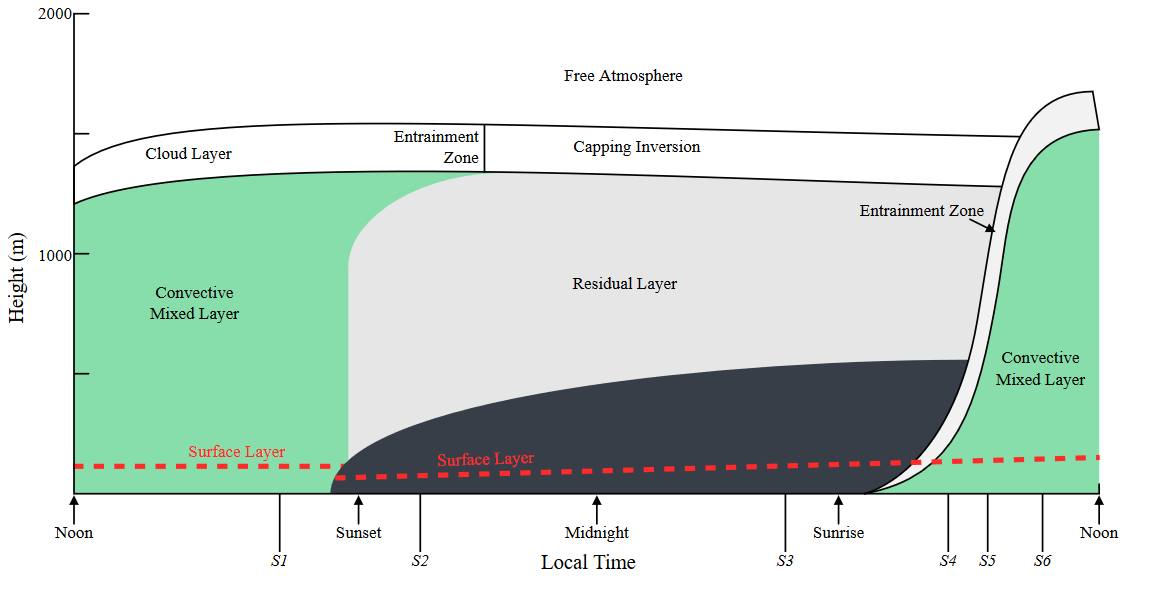
\includegraphics[width=10cm]{figures/PBL2.png}
        \caption{Diurnal cycle of vertical structure of the ABL, source: \url{https://www.weatherhawks.com/}.}
        \label{fig:pbl-diurnal}
    \end{figure}
    \item What are large-scale influence factors on the evolution and characteristics of the boundary layer? %\textit{Large-scale pressure gradients/wind/vertical motion, cloud cover, orography/orographically induced wind systems and surface properties/vegetation/water availability.}
    \item The surface layer is often described using Monin-Obukhov similarity theory (MOST). Explain the idea, assumptions and conclusions of MOST. %\textit{MOST assumes that turbulence is produced either mechanically or thermally and derives based on the assumption of a flat surface and a homogeneous flow, vertical profiles of all turbulent quantities just based on a dimensionless quantity, called stability parameter $\zeta = z/L$ with z the physical measurement height and L the Obukhov length.}
\end{enumerate}


\end{document}